%todo kapitel ändern!
\chapter{Frameworktest} \label{sec:test}
% testbackend muss noch geschrieben werden
% überlegungen zum testen aufschreiben 
Überprüfen der Funktionalität von den einzelnen Bestandteilen außerhalb der eigentlichen Anwendung gehört zum Entwickeln von Software dazu. %todo Quelle
Zusätzlich werden auch Tools zum Testen und Debuggen auf der Zielentwicklungsumgebung benötigt. 
In diesem Kapitel sollen beide Varianten näher betrachtet werden.


\section{Plattformunabhängige Tests}
Zunächst sollen auf die Tests eingegangen werden, die unabhängig von der Entwicklungsumgebung durchgeführt werden können. 
Damit dies möglich ist, muss die Struktur des \textit{fra\_handle} angepasst sowie ein entsprechendes Testbackend implementiert werden. Anschließend können verschiedene Tests erstellt werden, wobei die \gls{unittest} im Vordergrund stehen. Dadurch kann die \ac{fra} \gls{middleware} und Bibliothek unabhängig von der Software getestet und bei Änderungen überprüft werden, ob die beiden Teile korrekt arbeiten.

\begin{figure}[!hbtp]
	\centering
	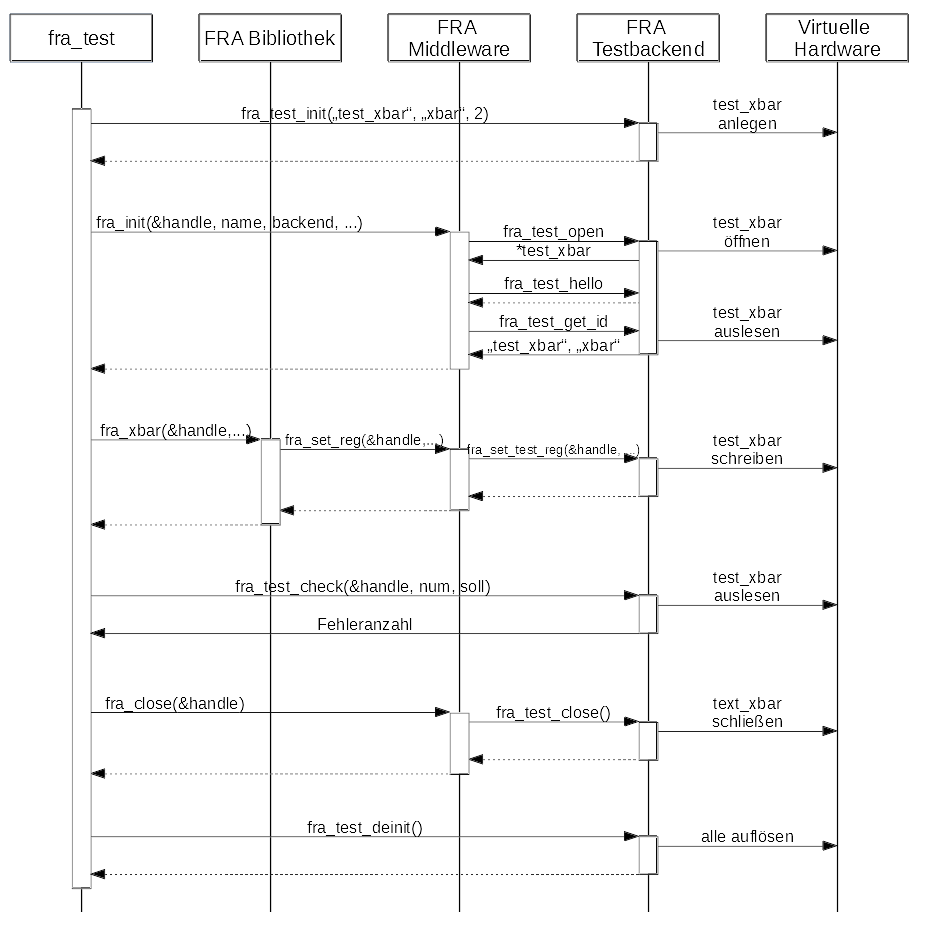
\includegraphics[width = \linewidth]{pictures/2019-11-28-testbackend.png}
	\smallskip
	\caption{Beispielhaftes Sequenzdiagramm zum \gls{unittest}}
	\label{fig:testbackend}
\end{figure} 


\begin{lstfloat}
\begin{lstlisting}
struct fra_test_mod
{
	char type[FRA_MAX_NAME];
	char name[FRA_MAX_NAME];
	uint32_t size;
	uint32_t *reg;
};
\end{lstlisting}
\captionof{code}{\label{code:fra_test_mod} Struktur zum Abbilden der vituellen Hardware}
\end{lstfloat}

Durch das Anlegen eines Geräts im Kernelbackend können alle benötigten Informationen und Register über dieses Gerät abgefragt und gesetzt werden. Da das Testbackend unabhängig laufen soll, ist das Anlegen von Geräten so nicht möglich. Um eine ähnliche Funktionalität wie im Kernel zu haben, wird das Modul über die \textit{fra\_mod\_test} Struktur abgebildet. Hier werden alle notwendigen Informationen angelegt und auch entsprechende Register abgebildet, damit man diese beschreiben und auch auslesen kann.
Die \textit{fra\_mod\_test} Struktur wird als statisches Array im Testbackend angelegt und bildet so die virtuelle Hardware für das Testprogramm. Dadurch ist das Überprüfen der Register später möglich und auch eine maximale Anzahl der Module ist vorgegeben. 


Damit die virtuelle Hardware richtig initialisiert wird, muss für die Register entsprechender Speicherplatz allokiert, aber auch die restlichen Parameter gesetzt werden. Analog dazu muss der Speicherbereich der Register beim Beenden des Programms wieder freigegeben werden. Dafür gibt es im Testbackend zusätzliche Funktionen, die sich um das initialisieren und deinitialisieren kümmern.\\

 
Beim Starten des Test wird der \textit{fra\_test\_init} Funktion drei Parameter übergeben. Zum Einen wird der Name sowie der Typ des Moduls und zum Anderen wird die Größe des Registers in die Funktion gereicht. Ist die maximale Anzahl der Module noch nicht überschritten, wird mithilfe der Größe ein Registerblock allokiert. Anschließend wird die \textit{fra\_mod\_test} Struktur mit allen vier Parametern gefüllt und eine statische Variable \textit{mod\_count} erhöht.

Wenn der Test am Ende angelangt ist, werden in der \textit{fra\_test\_deinit} Funktion mithilfe der Variablen \textit{mod\_count} alle allokierten virtuellen Geräte wieder freigegeben.\\


Zum Öffnen eines Moduls im Testbackend wird analog zum Kernelbackend die Funktion \textit{fra\_init} aufgerufen. Hier wird allerdings ein anderer Backendtyp übergeben und somit in den Wrapperfunktionen entsprechend ins Testbackend weitergeleitet. 
Die Funktionalität der einzelnen Backendfunktionen ist, im Vergleich zum Kernelbackend, vereinfacht worden und die Funktionen kommen entsprechend ohne \ac{ioctl}s aus. Das Setzen und Lesen der Register erfolgt nun über die \textit{fra\_mod\_test} Struktur im \gls{handle}. Diese wird bei der \textit{fra\_test\_open} Funktion als Zeiger auf die entsprechende Stelle im statischen \textit{fra\_mod\_test} Array beschrieben. Die richtige Stelle wird über einen Vergleich mit dem Modulname gefunden.\\



Damit überprüft werden kann, ob die Register richtig beschrieben bzw. ausgelesen worden sind, gibt es zwei Funktionen. Diese sind, wie die \textit{fra\_test\_init} und \textit{fra\_test\_deinit} Funktion, im Testbackend, aber werden ohne Wrapperfunktion aufgerufen, da sie spezifisch sind und lediglich beim Testen genötigt werden.
Der \textit{fra\_test\_check} Funktion werden neben dem \gls{handle} noch die Registernummer und der Sollwert des Registers übergeben. Über den Namen wird die Zuordnung des \glspl{handle} zu der virtuellen Hardware gemacht und anschließend der Registerwert mit dem Sollwert verglichen. Bei einem fehlerhaften Wert wird eine Fehlermeldung ausgegeben und der Rückgabewert ist 1.
Durch eine weitere Funktion (\textit{fra\_test\_check\_all}) kann das gesamte Register überprüft werden. Allerdings muss hier neben dem \gls{handle} noch ein Array der Registergröße übergeben werden. In diesem Array müssen die Sollwerte in richtiger Reihenfolge gespeichert sein. Anschließend wird für jede einzelne Registerstelle die \textit{fra\_test\_check} Funktion aufgerufen. Am Ende wird die Gesamtanzahl der Fehler zurückgegeben, welche im Test ausgewertet wird.\\


Im \gls{unittest} wird nun die virtuelle Hardware angelegt und geöffnet, anschließend werden modulspezifische Funktionen aufgerufen und direkt danach der Check durchgeführt (siehe Abbildung~\ref{fig:testbackend}). Dadurch kann die Funktionalität der einzelnen Module überprüft und im Fehlerfall direkt gehandelt werden. Vor allem bei Änderungen an der \ac{fra} Bibliothek können so vor der Inbetriebnahme auf der Kamera Fehler gefunden und ausgebessert werden.


\section{Tools für die Entwicklungsumgebung}
Unabhängig von der Funktionstests des vorherigen Kapitels sollten dem Entwickler kleine Programme zur Verfügung gestellt werden, mit denen man für Testprogramme oder zur Fehlersuche im laufenden Betrieb ein Gerät anlegen oder das Logging aktivieren kann.\\


Besonders für die Kalibrierung der Kamera ist es notwendig ein Gerät über die Kommandozeile anzulegen, da es hier keinen Codeteil gibt, in welchem das Anlegen integriert werden könnte. Dadurch das die benötigten Geräte vor dem Starten der Kalibiersoftware angelegt werden, können in der Software über die Funktionen der \ac{fra} \gls{middleware} und Bibliothek die Geräte geöffnet und auf diese zugegriffen werden.


Beim Ausführen des Programms \textit{fra\_create\_device} werden in der Kommandozeile über Optionen die benötigten Parameter übergeben. Hier gibt es, neben dem Namen, dem Typ, der Adresse und der Größe auch, die Möglichkeit eine Hilfe auszugeben, in welcher genauer erläutert wird, wie das Programm zu nutzen ist. 
Nach dem Ausführen des Programms werden die programminternen Parameter mithilfe der Optionen gefüllt und nach der Überprüfung auf Dateninkonsistenz wird das entsprechende Gerät angelegt. 
Danach ist dieses Gerät in Linux unter \textit{dev/fra/} zu finden und weitere Programme oder Testtools können darauf zugreifen.\\

Ein weiteres nützliches Tool für die Entwicklungsarbeit ist das \textit{fra\_set\_logging}. Da das Logging standardmäßig deaktiviert ist, muss dieses bei Bedarf aktiviert werden. Damit der Entwickler nicht im entsprechenden Code die Aktivierung vornehmen und zeitaufwendig neu kompilieren muss, wird durch das Testtool ein entsprechendes Werkzeug bereitgestellt. Durch das Programm kann im laufenden Betrieb der Kamera die Protokollierung eines Geräts aktiviert oder deaktiviert werden.


Hier werden beim Starten des Programms auf der Kommandozeile entsprechend den Optionen der Name des Geräts und ein Setparameter übergeben. 
Über den Setparameter wird entschieden, ob das Logging aktiviert (\textit{set=1}) oder deaktiviert (\textit{set=0}) werden soll. Anschließend wird das Gerät über den Namen geöffnet und über das entsprechende \ac{ioctl} wird das Logging gesetzt. Nach dem Schließen des Geräts wird das Programm beendet. \\


Beide Tools sind für den Einsatz auf der Entwicklungsumgebung gedacht und sollen Entwicklern und Testern vor allem die Fehlersuche auf der Kamera erleichtern. Bei Bedarf können die Programme einfach erweitert werden oder weitere Tools in Anlehnung an die Codestruktur geschrieben werden. 